% Rapport de cours ETA013. Les chiffres viennent du pipeline
% (data/processed/results.json) ; ce fichier les met en page.
\documentclass[11pt,a4paper]{article}

\usepackage[utf8]{inputenc}
\usepackage[T1]{fontenc}
\usepackage{lmodern}
\usepackage[english]{babel}
\usepackage{microtype}
\usepackage{amsmath}
\usepackage{booktabs}
\usepackage{tabularx}
\usepackage{array}
\usepackage{graphicx}
\usepackage{caption}
% Depuis docs/report/, les graphes sont deux niveaux au-dessus.
\graphicspath{{../../pictures/experiments/}}
\usepackage[margin=2.4cm]{geometry}
\usepackage{enumitem}
\usepackage{float}
\usepackage{fancyhdr}
\usepackage[hidelinks]{hyperref}

\setlist{itemsep=0.25em,topsep=0.4em,leftmargin=1.35em}
\captionsetup{font=small,labelfont=bf,skip=8pt}
\setlength{\parskip}{0.45em}
\setlength{\parindent}{0pt}

\hypersetup{
  pdftitle={Building energy study --- Danderyd},
  pdfauthor={Dimitri Marchand},
  pdfsubject={ETA013, Building Energy Systems, University of Gavle}
}

% Utilisable en texte et dans une équation.
\newcommand{\degC}{\ensuremath{^{\circ}\mathrm{C}}}
\newcommand{\WmK}{W/(m$\cdot$K)}
\newcommand{\WmTwoK}{W/(m$^{2}{\cdot}$K)}

\pagestyle{fancy}
\fancyhf{}
\fancyhead[L]{\small ETA013, University of G\"avle}
\fancyhead[R]{\small Dimitri Marchand}
\fancyfoot[C]{\thepage}
\renewcommand{\headrulewidth}{0.3pt}
\fancypagestyle{plain}{%
  \fancyhf{}%
  \fancyfoot[C]{\thepage}%
  \renewcommand{\headrulewidth}{0pt}%
}

\title{%
  Building energy study\\[0.35em]
  \large A multi-family building in Danderyd%
}
\author{%
  Dimitri Marchand\\
  \small Birth date 29 August 1986\\[0.35em]
  \small Course ETA013, Building Energy Systems\\
  \small University of G\"avle%
}
\date{12 October 2026}

\begin{document}
\maketitle
\thispagestyle{fancy}

\section{What the brief asks for}

A housing association has one multi-family building that cannot keep
20~\degC{} indoors when the weather is really cold. The brief asks for
the radiator power on a design day, the balance temperature, the average
$U$-value, the heating season in the city's weather file, and the energy
class once that year has been brought back to a normal climate.

The birth date is 29~August 1986. Written as year, month, day
(1986, 08, 29) it gives $a = 0$, $b = 8$, $c = 2$, $d = 9$, $ab = 8$,
$cd = 29$, the same split as the example in the brief
(1985, 10, 29 gives $a = 1$, $b = 0$, $c = 2$, $d = 9$).
Indoor setpoint $T_{\mathrm{in}} = 20 + c = 22.0$~\degC.
The heating system is an air-to-air heat pump, COP~3.

\begin{table}[ht]
\centering
\caption{Answers the brief asks for.}
\label{tab:answers}
\begin{tabularx}{\textwidth}{@{}>{\raggedright\arraybackslash}X r@{}}
\toprule
Quantity & Value \\
\midrule
City & Danderyd (number 29) \\
DVUT & $-10.7$~\degC{} (7-day) \\
Indoor temperature $T_{\mathrm{in}}$ & 22.0~\degC \\
Average heat transfer coefficient $U_m$ & 0.589~\WmTwoK \\
Balance temperature $T_b$ & 18.21~\degC \\
Heating power, no internal gains & 46.5~kW \\
Same power, appliance gains only & 41.1~kW \\
Heat gain, people & 3.8~kW, 22.2~MWh \\
Heat gain, appliances & 5.4~kW, 31.5~MWh \\
Solar heat gain & 19.9~MWh \\
Heat loss, transmission & 109.0~MWh \\
Heat loss, ventilation & 43.6~MWh \\
Heat deficit, weather year 2017 & 80.2~MWh \\
Degree hours, base $T_{\mathrm{in}}$ & 107\,242~\degC$\cdot$h \\
Heat deficit, normal-year correction & 81.7~MWh \\
Primary energy number & 108.3~kWh/m$^{2}{\cdot}$year \\
Energy class & E \\
\bottomrule
\end{tabularx}
\end{table}

Seasonal energies in Table~\ref{tab:answers} cover the heating season
(15~September to 15~May). The duration diagram of the outdoor temperature
is Figure~\ref{fig:duration}.

\section{The building}

Three storeys ($3 + a$), plan $10 \times 45$~m.
Heated floor area $A_{\mathrm{temp}} = 1\,350$~m$^{2}$.
Storey height 2.5~m, so the heated volume is $3\,375$~m$^{3}$.
The brief gives the plan as $10 \times 45$~m$^{2}$ and no internal
dimensions, so $A_{\mathrm{temp}}$ is that plan times the number of storeys.

Gross fa\c{c}ade 825~m$^{2}$, of which windows 129.0~m$^{2}$
and doors 50.4~m$^{2}$. Opaque wall left: 645.6~m$^{2}$.
The enclosing area $A_{\mathrm{om}}$ is 1\,725~m$^{2}$
(roof + ground floor + whole fa\c{c}ade, windows and doors included).

External corridors run along both long sides, on the intermediate floors.
With two intermediate floors and two sides of 45~m, the thermal-bridge
length is 180~m at $\Psi = 0.6$~\WmK.

\section{U-value of the outer wall}
\label{sec:wall}

The brief asks for the $\lambda$-value method. The studs are 45~mm wide
at 600~mm centres, so the wood fraction is $45/600 = 0.075$.
Mineral wool is 0.037~\WmK{} and timber is 0.14~\WmK:
\begin{equation}
  \lambda_{\mathrm{mix}}
  = 0.925 \times 0.037 + 0.075 \times 0.14
  = 0.0447~\mathrm{W/(m{\cdot}K)}.
  \label{eq:lambda}
\end{equation}

The ventilated cavity and the outer leaf (the brick) are given as one
resistance, 0.20~m$^{2}{\cdot}$K/W. Asbestos and the plastic foil are
ignored, as the brief says. Indoor surface resistance is the usual
0.13~m$^{2}{\cdot}$K/W for a wall. Gypsum is 13~mm at 0.25~\WmK.
\begin{equation}
  R = 0.13 + \frac{0.013}{0.25} + \frac{0.095}{\lambda_{\mathrm{mix}}} + 0.20
    = 2.506~\mathrm{m^{2}{\cdot}K/W},
  \label{eq:rwall}
\end{equation}
so $U_{\mathrm{wall}} = 1/R = 0.399$~\WmTwoK.
Horizontal noggins are not given, so they are not included.
Counting them would raise $U$ a little.

\section{Average heat transfer coefficient}
\label{sec:um}

$U_m$ is the transmission heat loss, bridges included, divided by
$A_{\mathrm{om}}$. Ventilation is not part of $U_m$.

\begin{table}[ht]
\centering
\caption{Transmission coefficients. Windows are double glazing in timber
frames.}
\label{tab:um}
\begin{tabular}{@{}lr@{}}
\toprule
Part & $UA$ or $\Psi L$ (W/K) \\
\midrule
Opaque walls & 257.6 \\
Windows, $U = 2.9$~\WmTwoK & 374.1 \\
Doors, $U = 2.0$~\WmTwoK & 100.8 \\
Roof, $U = 0.16$~\WmTwoK & 72.0 \\
Ground floor, $U = 0.23$~\WmTwoK & 103.5 \\
Balcony slabs, $\Psi L$ & 108.0 \\
\midrule
Total $H_{\mathrm{tr}}$ & 1\,016.0 \\
\bottomrule
\end{tabular}
\end{table}

\begin{equation}
  U_m = H_{\mathrm{tr}} / A_{\mathrm{om}}
      = 1\,016.0 / 1\,725
      = 0.589~\mathrm{W/(m^{2}{\cdot}K)}.
  \label{eq:um}
\end{equation}
A new multi-family building in BBR is limited to 0.40~\WmTwoK.
This envelope is above that limit. The windows alone are a large part
of $H_{\mathrm{tr}}$.

\section{Ventilation}

Thirty-eight people is $30 + ab$. Each produces 0.005~L/s of CO\textsubscript{2},
outdoor air is 350~ppm, and the indoor limit used for sizing is 1\,000~ppm.
Parts per million is a volume fraction, so the difference is multiplied
by $10^{-6}$.
\begin{equation}
  q = \frac{38 \times 0.005~\mathrm{L/s}}{(1\,000 - 350)\times 10^{-6}}
    = 292~\mathrm{L/s}
    = 0.22~\mathrm{L/(s{\cdot}m^{2})}.
  \label{eq:vent}
\end{equation}
Leakage is 0.05 air changes per hour, 47~L/s. The system is mechanical
exhaust, so there is no heat recovery. For a design-day calculation the
two flows are added: that is the cold-day case, outdoor air coming in
both through the vents and through the cracks.
\begin{equation}
  H_{\mathrm{vent}}
  = 1.2~\mathrm{kg/m^{3}} \times 1\,000~\mathrm{J/(kg{\cdot}K)} \times q
  = 407.0~\mathrm{W/K}.
  \label{eq:hvent}
\end{equation}
The specific flow from the CO\textsubscript{2} balance is below the
0.35~L/(s$\cdot$m$^{2}$) often used as a hygienic floor for housing.
The brief says to size from the CO\textsubscript{2} measurement, so the
lower flow is kept. Raising it to 0.35 would increase the ventilation
loss, and the heating power with it.

\section{Time constant and DVUT}

DVUT is not the coldest hour of one year. It is the outdoor temperature
of a cold spell whose length matches the building's time constant.
Only the mass on the warm side of the insulation counts, and only the
first 10~cm from each indoor face (ISO~13790). The brick sits outside
the insulation, so it is left out. Using the whole 200~mm ground slab
would pretend that the soil-side concrete follows the room temperature.

The active capacity is $C = 822$~MJ/K. With
$H = H_{\mathrm{tr}} + H_{\mathrm{vent}}$:
\begin{equation}
  \tau = C / H = 6.69~\mathrm{days}.
  \label{eq:tau}
\end{equation}
Rounded to the nearest tabulated duration, that is the 7-day DVUT for
Danderyd: $-10.7$~\degC{} (Boverket / SMHI, 1991--2020).

\section{Balance temperature and design power}

$T_b$ is the outdoor temperature at which appliance gains alone cover the
losses. People and sun are left out, as the brief asks for $T_b$ and for
the design power.
\begin{equation}
  T_b = T_{\mathrm{in}} - \frac{Q_{\mathrm{appliances}}}{H_{\mathrm{tr}} + H_{\mathrm{vent}}}
      = 22.0 - \frac{5\,400}{1\,423}
      = 18.21~\degC.
  \label{eq:tb}
\end{equation}
Above $T_b$ the building does not need the radiators, if the appliances
are running and sun and people are still ignored. Below $T_b$ it does.

The question on power without internal heat generation is the full loss
at DVUT. The hint then says to keep the appliances. Both numbers are
reported. The safe size of the heating system is the larger one:
appliances are not a guarantee at six in the morning.
\begin{align}
  P &= (H_{\mathrm{tr}} + H_{\mathrm{vent}}) \times (T_{\mathrm{in}} - \mathrm{DVUT})
    = 46.5~\mathrm{kW}, \label{eq:power}\\
  P - Q_{\mathrm{appliances}} &= 41.1~\mathrm{kW}. \nonumber
\end{align}

On that design day the loss splits as in Figure~\ref{fig:shares}
and Table~\ref{tab:shares}.

\begin{table}[ht]
\centering
\caption{Design-day heat loss at DVUT, $T_{\mathrm{in}} = 22$~\degC.}
\label{tab:shares}
\begin{tabular}{@{}lr@{}}
\toprule
Path & Power (kW) \\
\midrule
Ventilation and leaks & 13.3 \\
Windows & 12.2 \\
Outer walls & 8.4 \\
Balcony slabs & 3.5 \\
Ground floor & 3.4 \\
Doors & 3.3 \\
Roof & 2.4 \\
\bottomrule
\end{tabular}
\end{table}

\begin{figure}[H]
\centering
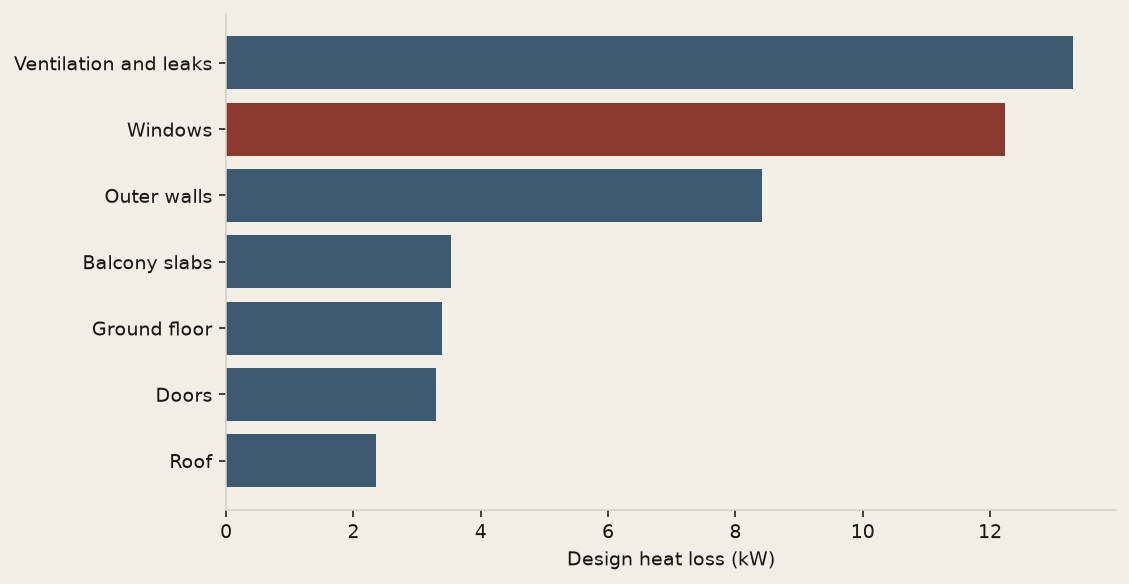
\includegraphics[width=0.78\textwidth]{design-power-shares.png}
\caption{Where the design-day heat leaves the building.
Ventilation is slightly ahead of the windows.}
\label{fig:shares}
\end{figure}

\section{Heating season, 15 September to 15 May}

The weather file is Sveby / SMHI for Danderyd, 2017
($2015 + a + a + c$). Solar radiation is the monthly curve printed in
the brief (\"Orebro, 60$^{\circ}$~N), used for every city as instructed.
It was read from the printed figure to about $\pm 5$~W/m$^{2}$.
The values are monthly averages, so they are applied to every hour of
the month and then multiplied by the hours, as the hint in the brief says.

People contribute 3.8~kW: 38~people $\times$ 100~W.
The CO\textsubscript{2} rate in the brief, 0.005~L/s per person, is about
one met, which is about 100~W of heat. Presence is taken as continuous.
A real schedule, with people out during the day, would lower this gain.

Each hour,
\begin{equation}
  Q_{\mathrm{heat}}
  = \max\bigl(0,\;
      H_{\mathrm{tr}}(T_{\mathrm{in}} - T_{\mathrm{out}})
    + H_{\mathrm{vent}}(T_{\mathrm{in}} - T_{\mathrm{out}})
    - Q_{\mathrm{app}} - Q_{\mathrm{people}} - Q_{\mathrm{solar}}
    \bigr).
  \label{eq:hour}
\end{equation}
Surplus in a mild hour is not saved for the next hour.
There is no utilisation factor: gains are fully useful until they match
the loss. That is slightly optimistic.

The season is 5\,832~hours.
Degree hours with base $T_{\mathrm{in}}$: 107\,242~\degC$\cdot$h.
Degree hours with base $T_b$, used for the climate correction:
85\,117~\degC$\cdot$h in 2017 and 86\,725~\degC$\cdot$h in the typical year.

\begin{figure}[H]
\centering
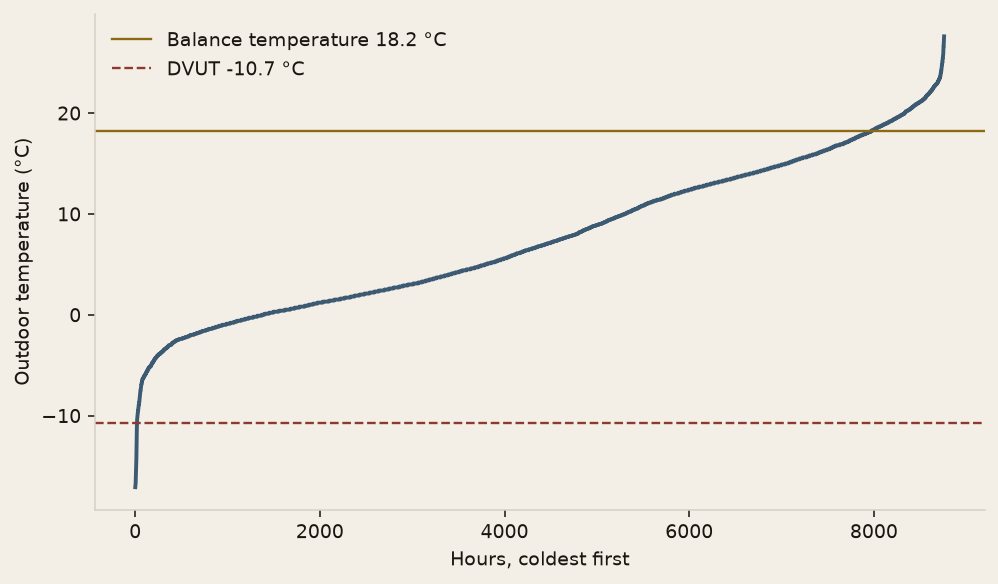
\includegraphics[width=0.92\textwidth]{duration-temperature.png}
\caption{Outdoor temperature in Danderyd, all hours of 2017, sorted
from cold to mild. Solid line: balance temperature. Dashed line: DVUT.}
\label{fig:duration}
\end{figure}

\begin{figure}[H]
\centering
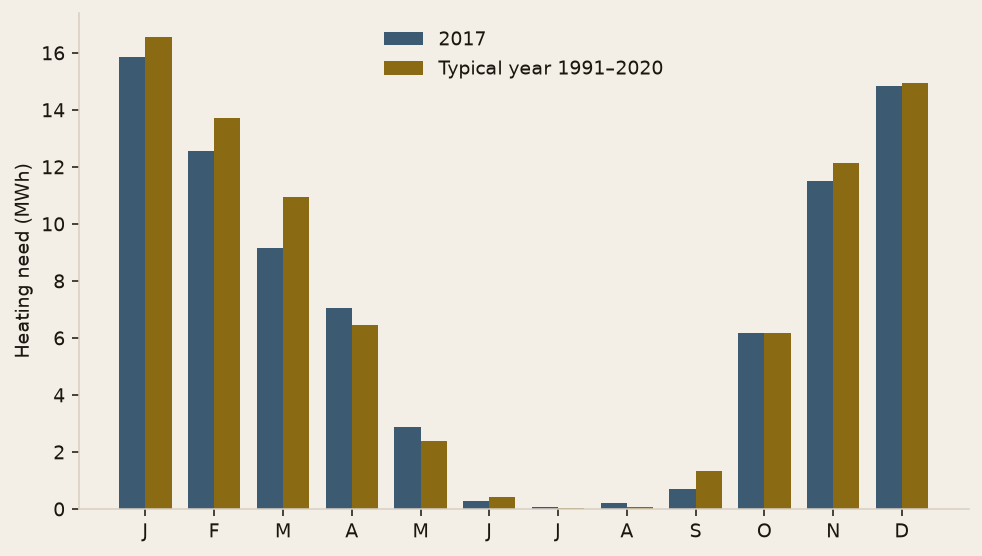
\includegraphics[width=0.92\textwidth]{monthly-heating.png}
\caption{Heating need by calendar month. 2017 beside the typical year
1991--2020. Summer months stay near zero.}
\label{fig:monthly}
\end{figure}

\section{Normal year and energy class}

The lecture correction scales the climate-dependent heat with the ratio
of degree hours (base $T_b$) between the typical year and 2017:
\begin{equation}
  E_{\mathrm{normal}}
  = E_{2017} \times \frac{\text{degree hours}_{\mathrm{normal}}}
                         {\text{degree hours}_{2017}}
  = 80.21~\mathrm{MWh} \times 1.019
  = 81.72~\mathrm{MWh}.
  \label{eq:normal}
\end{equation}
Running the same hourly balance on the Sveby typical year (1991--2020)
gives 83.08~MWh directly. The two routes are close. The energy class
below uses the scaled 2017 result, which is the correction the brief
points to. The direct run is the check.

The heating system is an air-to-air heat pump with COP~$= 3$.
Electricity bought for space heat is the heat divided by~3.
An air-to-air unit does not heat domestic hot water, so hot water is
counted as direct electric (25~kWh/m$^{2}$, Sveby).
Property electricity (fans, common lighting) is 15~kWh/m$^{2}$, also
Sveby, also electricity. Household appliances are already inside the
heat balance as a gain; their electricity is not part of the building's
primary energy number.

Weighting factors are the BBR ones: electricity 1.8, district heating
would have been 0.7. Only space heating is divided by the geographical
factor $F_{\mathrm{geo}}$. For Danderyd, $F_{\mathrm{geo}} = 1.0$, so the
factor does not move the number.
\begin{equation}
  \mathit{EP}
  = \frac{E_{\mathrm{heat}} \times 1.8 / F_{\mathrm{geo}}
        + E_{\mathrm{DHW}} \times 1.8
        + E_{\mathrm{property}} \times 1.8}
       {A_{\mathrm{temp}}}
  = 108.3~\mathrm{kWh/(m^{2}{\cdot}year)}.
  \label{eq:ep}
\end{equation}
Of that, space heating is 36, domestic hot water is 45, and property
electricity is 27, all in kWh/m$^{2}{\cdot}$year.
The heat pump divides the space-heat bill by three, so the hot-water
cylinder, still a plain electric heater, weighs more in the rating than
the heating does.

The new-building limit for a multi-family house is
75~kWh/m$^{2}{\cdot}$year. There is no ventilation supplement: the
specific flow is under 0.35~L/(s$\cdot$m$^{2}$).
The ratio is 1.44, which is energy class~E
(Figure~\ref{fig:class}).

Class~C means as good as the requirement for a new building.
Classes toward~A are better. This building does not meet that requirement.
Most of the primary energy is electricity, and electricity is weighted
at~1.8. The same heat on district heating (weight 0.7, no COP) would
look different. The birth date fixes the system, so that comparison is
not the result, only a reminder that the class is about the carrier as
well as the heat.

One limit of the COP: it is taken as~3 even on the design day.
A real air-to-air pump loses capacity in a cold spell.
The design power above is the heat the building needs.
The pump may need a backup heater to deliver it at DVUT.
That backup is not in the annual COP of~3, so the annual electricity,
and the class, are a little optimistic.

\begin{figure}[H]
\centering
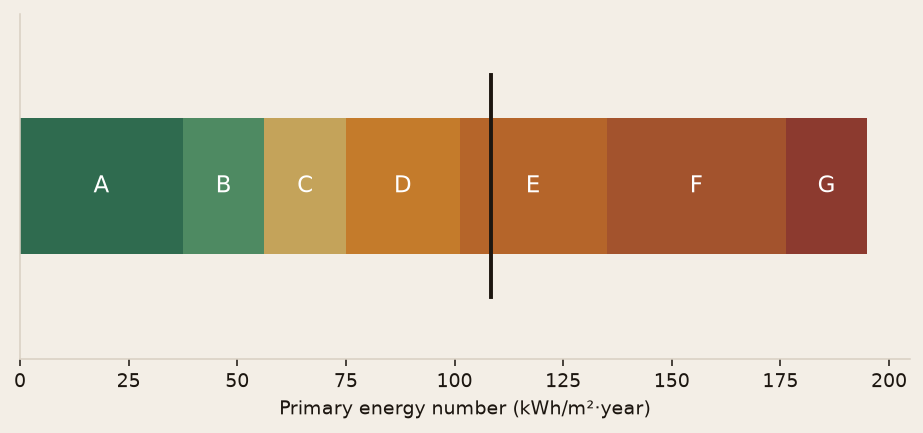
\includegraphics[width=0.86\textwidth]{energy-class.png}
\caption{Primary energy against the BBR class boundaries for a new
multi-family building. The result sits in class~E.}
\label{fig:class}
\end{figure}

\section{What would actually cut the heating}

Each line in Table~\ref{tab:measures} repeats the normal-year correction
with one change applied.

\begin{table}[ht]
\centering
\caption{Measures, same climate correction as the base case.}
\label{tab:measures}
\begin{tabular}{@{}lrrr@{}}
\toprule
Measure & Heat (MWh) & Saved (MWh) & Class \\
\midrule
Triple glazing, $U = 1.0$~\WmTwoK & 56.2 & 25.5 & D \\
Heat recovery, 80\,\% of exhaust air & 52.6 & 29.2 & D \\
Balcony break, $\Psi = 0.20$~\WmK & 74.2 & 7.6 & E \\
All three together & 22.1 & 59.6 & D \\
\bottomrule
\end{tabular}
\end{table}

The order of usefulness, on this building:

\begin{enumerate}
  \item \textbf{Heat recovery on the exhaust air.}
        The ventilation loss is large and today it is thrown away.
        An exhaust-air heat pump, or a supply-and-exhaust unit with
        80\,\% recovery, attacks that term directly.
        Leakage is left unchanged.
  \item \textbf{The windows.}
        $U = 2.9$ on more than 100~m$^{2}$ is the biggest single
        transmission term. Triple glazing around $U = 1.0$ is the
        obvious replacement.
  \item \textbf{The balcony slabs.}
        $\Psi = 0.6$~\WmK{} over the long fa\c{c}ades is a serious
        bridge, which the brief already flags. A thermal break at the
        slab edge cuts it without touching the apartments much.
\end{enumerate}

Doing all three still leaves domestic hot water and property electricity,
both counted as electricity at factor~1.8. Together those two terms are
about 72~kWh/m$^{2}{\cdot}$year before any space heat is added.
The class moves from~E to~D, but the envelope alone does not reach
class~C, because the primary-energy number is not only the space heating.

\section{What this does not claim}

\begin{itemize}
  \item The city list was not inside the PDF. City~29 is Danderyd because
        the SMHI place list, without Abisko, puts Bjurholm at number~14
        (a known reading of the same brief) and Danderyd at number~29.
  \item The solar chart in the brief was read by eye. A few watts per square
        metre either way does not change the class; it does move the
        solar megawatt-hours.
  \item Internal gains other than the constant 100~W per person and the
        appliance wattage are not modelled. No night setback, no shutters.
  \item The 10~cm active-depth rule is used only to pick DVUT. The annual
        energy calculation is steady-state, hour by hour, not a dynamic
        simulation.
  \item Hot water and property electricity are Sveby standard values, not
        measurements from this association.
  \item The mean outdoor temperature in 2017 was 7.65~\degC, against
        7.32~\degC{} in the normal year, so 2017 was slightly milder.
        The coldest hour of 2017 ($-17.1$~\degC) is colder than the
        1-day DVUT ($-13.5$~\degC). DVUT is a sustained spell, not the
        coldest hour.
\end{itemize}

\begin{thebibliography}{9}
\bibitem{brief}
  Assignment brief, course ETA013, University of G\"avle.
  Deadline 17~November 2026.

\bibitem{dvut}
  Boverket / SMHI, DVUT 1991--2020, open data.
  Place Danderyd, ortnr 102646.

\bibitem{sveby2017}
  Sveby climate file for 2017, version 2.0, place Danderyd (102646).

\bibitem{svebytyp}
  Sveby typical year 1991--2020, same place.
  Composite year: the month and hour columns are used, not the source year.

\bibitem{fukth}
  Figure~1 of the brief: Nevander and Elmarsson,
  \emph{Fukthandboken}, 1994. Monthly solar irradiance at \"Orebro, 60$^{\circ}$~N.

\bibitem{bbr}
  Boverket, BBR: electricity weighting factor 1.8,
  new multi-family limit 75~kWh/m$^{2}{\cdot}$year, classes A--G.
  $F_{\mathrm{geo}} = 1.0$ for Danderyd.

\bibitem{svebyuse}
  Sveby user input data for multi-family buildings:
  domestic hot water 25~kWh/m$^{2}{\cdot}$year,
  property electricity 15~kWh/m$^{2}{\cdot}$year.

\bibitem{iso13790}
  ISO~13790, 10~cm active depth for the thermal mass used to select DVUT.
\end{thebibliography}

\end{document}
